\subsection{Signal Extraction}
Once the excess noise has been diminished, the gravitational wave signal needs to be identified and pulled. Excess power and Template matching are some of the more frequently used methods to identify and extract the signals.

\subsubsection*{Excess power method}

The “excess power” method is much enhanced when several detectors are employed. With it, the data streams from each observatory are searched for signals that are not easily accounted for by the noise characteristics of that particular instrument. When such interesting signals are found, corresponding signals, using an appropriate time window, are searched for in the data from the other observatories. Essentially, the signals from the different detectors are cross-correlated with each other. Since the noise in each experiment is uncorrelated with that of the others, a real signal should give a large spike in the correlation statistic. Complicating the analysis is the sensitivity of the detectors to the direction to the source, which can weaken the signal in one observatory relative to the others. But this effect can be taken into account and poses no serious problem.

\subsubsection*{Template matching}

Another method to find gravitational waves is to look for signals that coincide with events that are visible using other means, and that should also emit gravitational waves. The first step in computing a template signal is computing the gravitational wave signature of different astrophysical sources. While template matching is a powerful way to extract a gravitational wave signal from the noise, it only works for sources that can be easily modelled. \\

The models compared to the LIGO data are called phenomenological models, and they are fit to numerical simulations of systems created by solving the Einstein equation on supercomputers. A smaller number of simulations are computed, and then an analytic model is created that links one simulation to another. A set of freely adjustable parameters is used with these models that allow them to match all of the available numerical simulations and to interpolate between them. There are several models that are used for this. Each uses a slightly different method, and so they produce slightly different wave forms. The implied properties of the modelled systems also differ as a result, but only in small ways. However, template matching alone would result in a lot of spurious matches and random data fluctuations.

\begin{figure}[h]
    \centering
    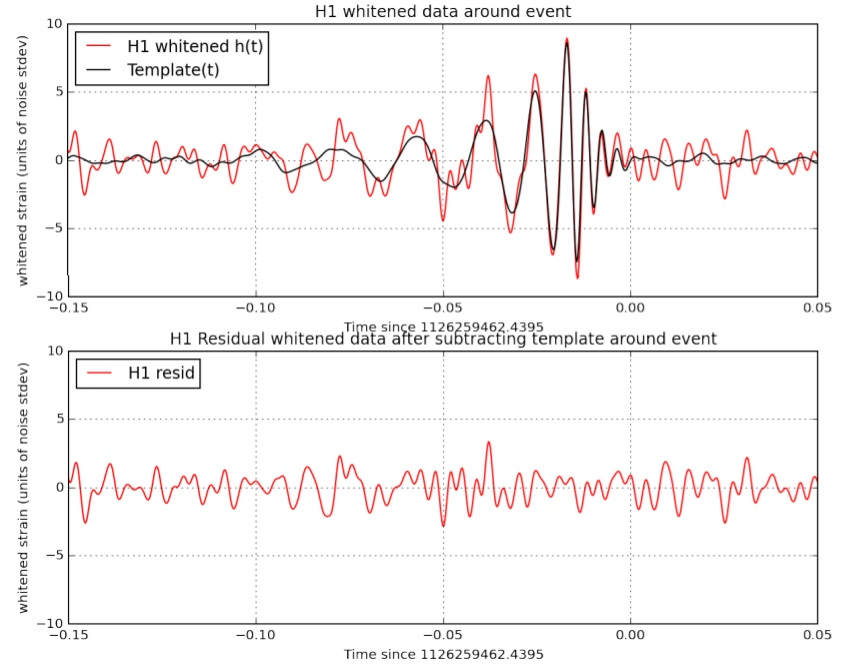
\includegraphics[scale=0.92]{images.tex/template_matching.jpg}
    \caption{Matching the received signal using Gravitational waveform as a template.\\ Source :- \href{https://kiss.caltech.edu/workshops/LISA/presentations/Babak.pdf}{Introduction to Data Analysis of Gravitational Wave Signals by Stanislav Babak}}
\end{figure}

Therefore, we need to apply a “SNR” filter13, taking only the samples above some threshold value of the signal-to-noise ratio. In the LIGO data, it turns out that if one sample has a high SNR, then it is usually surrounded by neighbors that also have high SNR. Most of these are false positives and LIGO performs yet another cut, keeping only the single highest SNR candidate in each such cluster. This further reduces the size of the data set. After that, the software looks for coincidence between the two LIGO antennas. From the reduced data set, a statistic called the log likelihood ratio, or LLR is computed . The larger the LLR for a candidate, the more likely it is to be caused by a signal rather than noise, and vice versa. When a real signal is present in the data, it is generally surrounded by a large number of candidates which are the result of matches by similar-shaped templates to the matching one. This has been determined by many runs in which simulated waveform data have been injected into the data stream to test the software. \\

This allows candidates to be clustered, similar to the way the SNR threshold peaks were clustered; in this case, if a candidate falls within 4 seconds of another candidate that has a higher LLR, the weaker candidate is discarded. It turns out that there is a high probability of finding a low-ranked candidate next to a high ranked one, and so this method successfully trims many low ranked candidates from the sample. However, for candidates with LLR larger than about 6, this clustering method is not effective because the probability of two such candidates being within 4 seconds of one another so low: the recent data run produced one candidate like this about every 5 minutes, or 10, 000 of them for the entire run. The total sample in the data set has now been reduced from 500 million per second to only 10, 000 total, a small enough sample that it is possible to perform detailed statistical testing on each one of them.\\

Once the GW signal is extracted, then it's frequency will be changed by multiplying it with a conversion ratio, such that the resulting frequency lies in the audible range. On September 14 2015, the first characteristic `chirp' sound of the GW150914 was decoded using LIGO. 

\pagebreak
